%!TEX root=./LIVRO.tex
\chapter{Água}
\markboth{Módulo 1}{}

\vspace*{-1.5cm}
\enlargethispage{4\baselineskip}

\section*{Eixo de conhecimento do SAEB}
\begin{itemize}
	\item Matéria e energia.
\end{itemize}

\subsection{Habilidades da BNCC}

\begin{itemize}
\item EF05CI02, EF05CI03, EF05CI04.
\end{itemize}

\conteudo{A água presente na superfície da Terra se recicla há 
milhões de anos. 

Porções de água se movimentam ao redor do planeta, sem parar: é o 
\textbf{ciclo hidrológico da água}, que acontece por causa das 
mudanças de estado físico e é influenciado pelas movimentações 
da água na natureza ou realizadas pelos seres humanos. 

\begin{wrapfigure}{l}{.5\textwidth}

\includegraphics[width=.5\textwidth]{./imgs/img16.jpg}
\end{wrapfigure}
%\caption{https://br.freepik.com/vetores-gratis/dia-mundial-da-agua-desenhado-a-mao_12338724.htm#query=%C3%A1gua%20Planeta%20Terra&position=1&from_view=search&track=ais}

Nesse ciclo, a água é naturalmente reciclada, ao ser evaporada
de solos e rios, transpirada pela vegetação e condensada nas nuvens,
para então se precipitar e cair de volta na superfície sob a
forma de chuva. Ele pode ser alterado, a depender da realidade de 
cada região, dos hábitos da população, da preservação ambiental e
dos fenômenos naturais.

Em algumas situações, o funcionamento do ciclo hidrológico da água é
alterado por características naturais ou pela ação
humana. Problemas como a baixa qualidade dos solos, o desmatamento
e a poluição atuam na potencialização do \textbf{assoreamento dos rios}
— isto é, o depósito de sedimentos no fundo das águas —, que pode 
mudar cursos d'água, causar inundações ou mesmo inviabilizar a
sobrevivência de espécies marinhas.

Para garantir a preservação de condições ambientais adequadas, 
deve-se atentar para os usos conscientes da água, tanto em atividades
comuns do dia a dia, como escovar os dentes, tomar banho e lavar
calçadas, quanto em observar os usos do recurso natural na produção 
agrícola e industrial de larga escala.}

\section*{Atividades}

\num{1} Indique, nos retângulos vazios, o nome das mudanças de
estado físico no ciclo hidrológico da água.

\begin{figure}[htpb!]
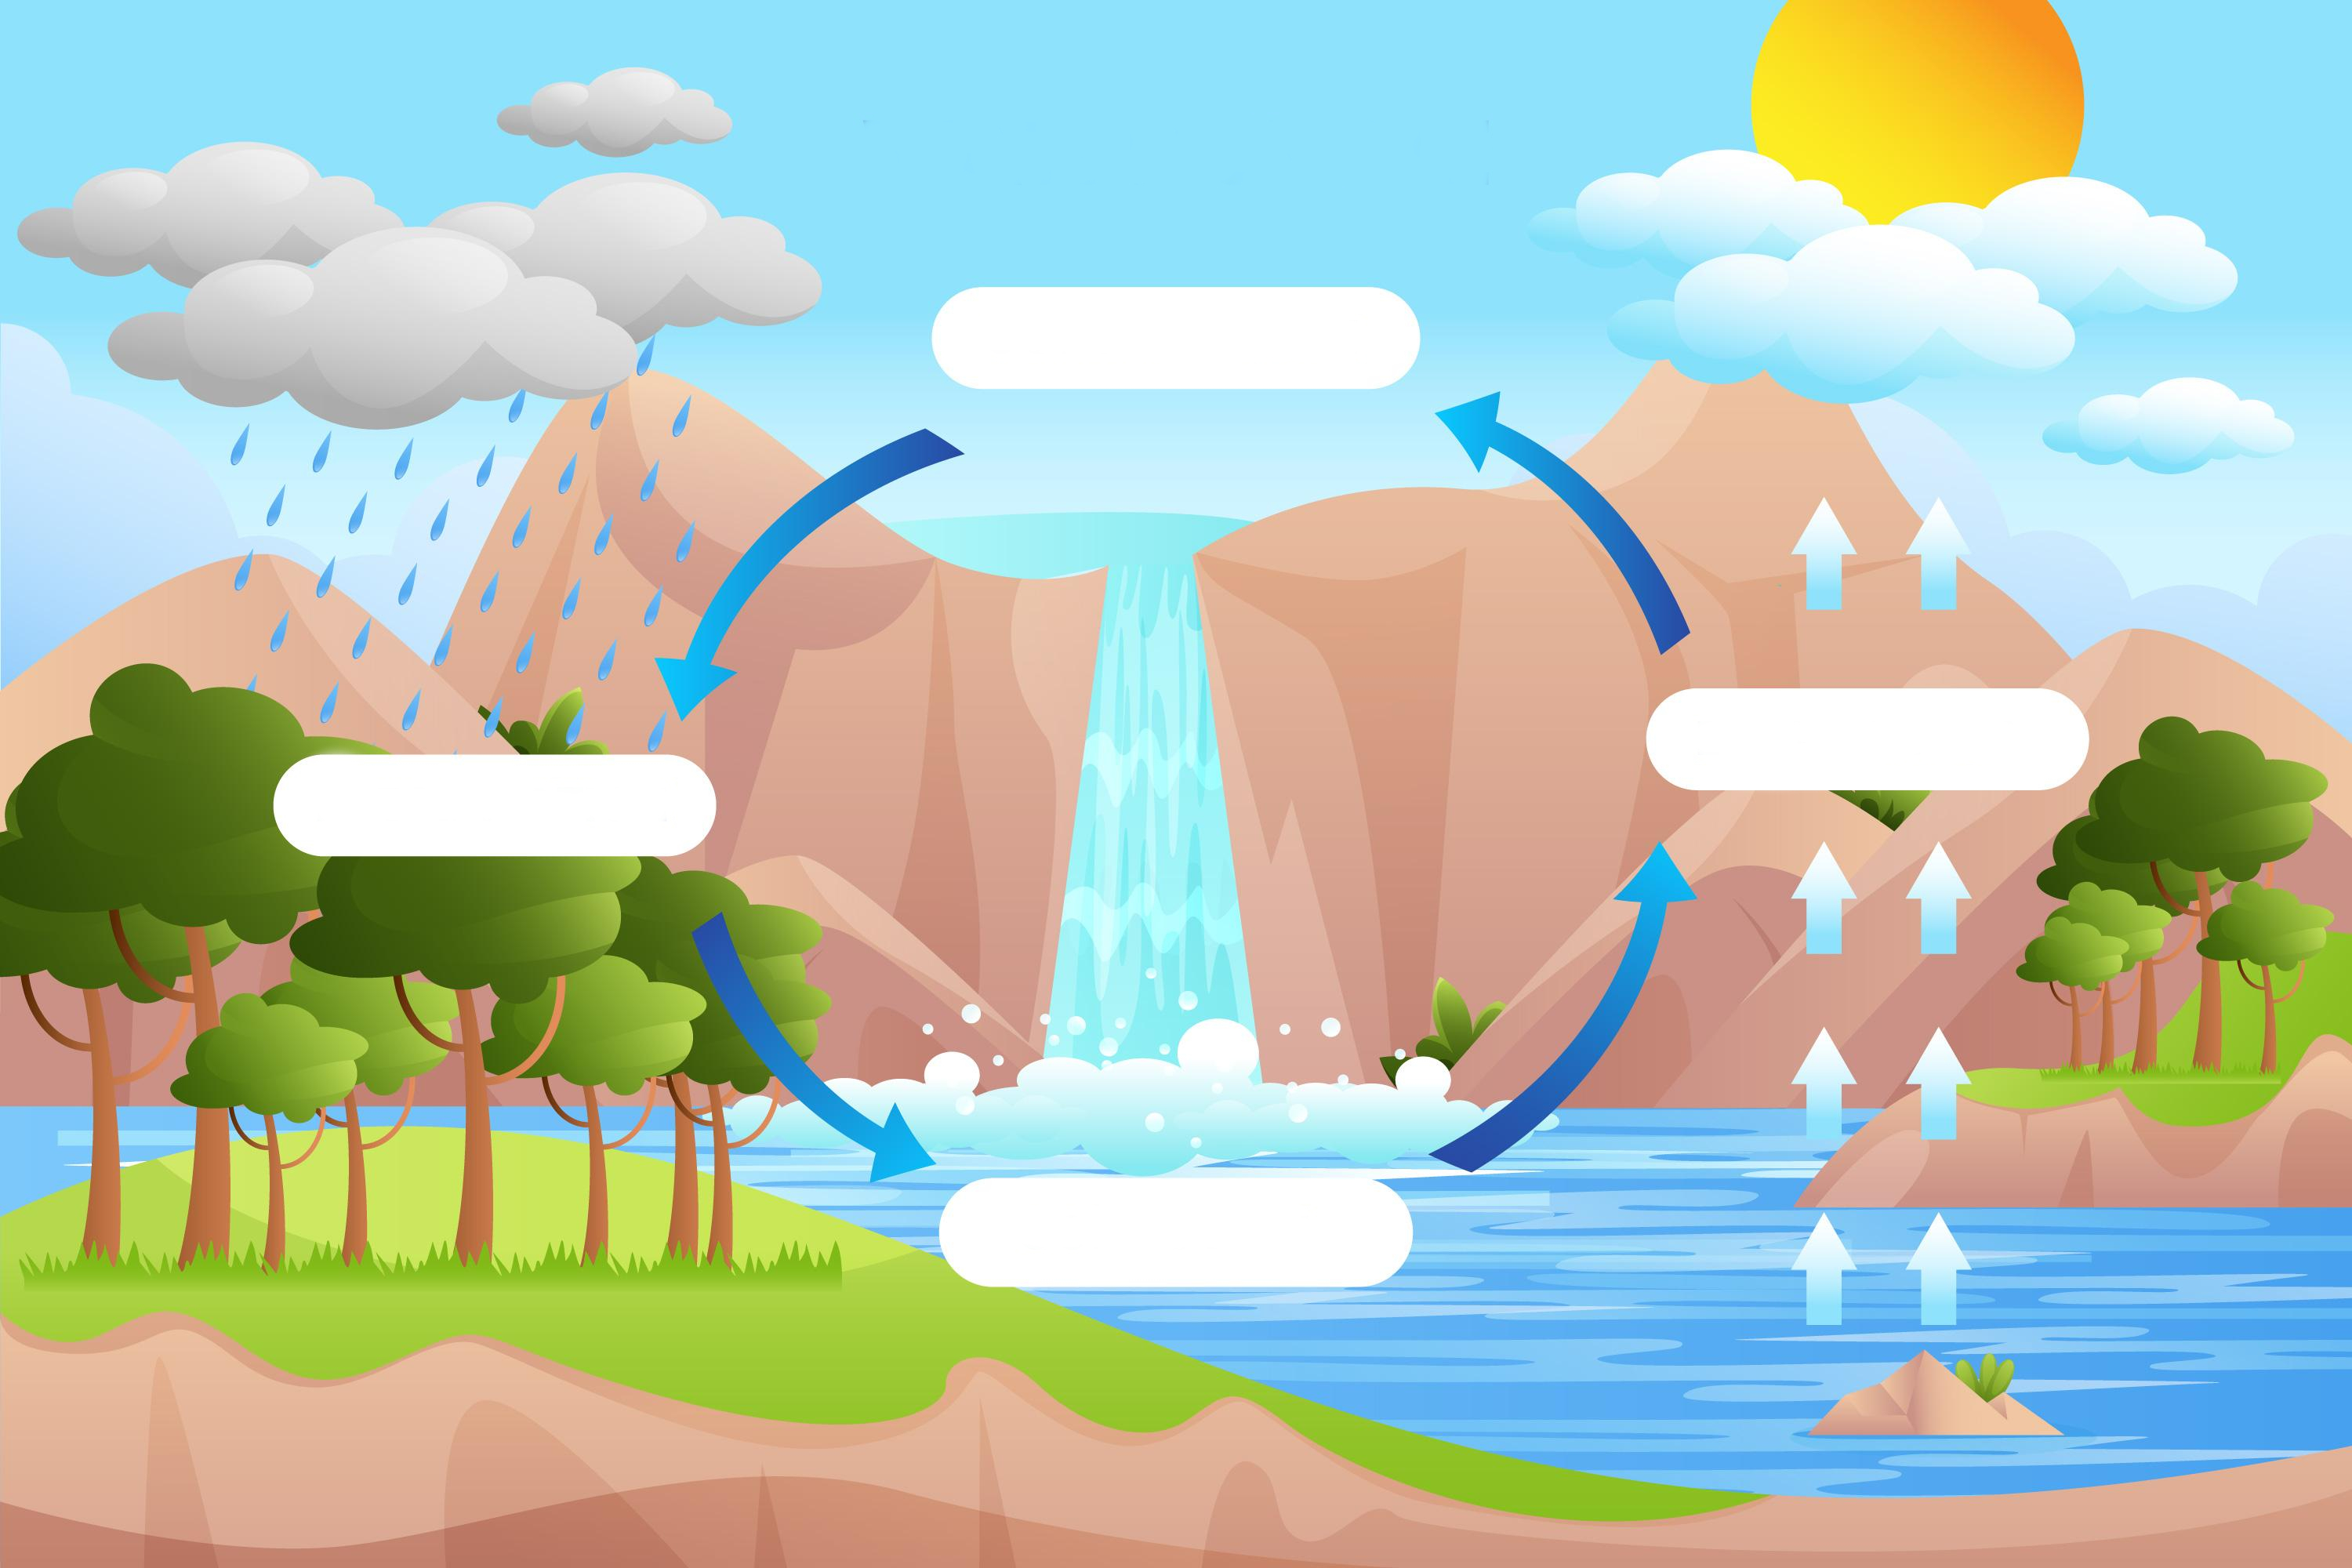
\includegraphics[width=\textwidth]{./imgs/img17.jpg}
%\caption{https://br.freepik.com/search?format=search&query=ciclo%20da%20%C3%A1gua}
\end{figure}

\coment{O calor gerado pelos raios solares aquece a água dos
oceanos e a água armazenada nos solos, levando ao fenômeno da 
\textit{evaporação}, além de atuar na transpiração das árvores que absorvem
a água do solo — a chamada \textit{transpiração} ou \textit{evapotranspiração}. Ocorre \textit{condensação} quando as nuvens se carregam dos vapores
d'água, até que as gotículas se agreguem e caiam na
superfície terrestre: é a \textit{precipitação}.}

\num{2} Relacione as colunas, indicando o uso da água de acordo com
a atividade correspondente.

\begin{multicols}{2}
\red{Irrigação} \rosa{agricultura}

\red{Limpeza de casa} \rosa{uso doméstico}

\red{Produção de energia} \rosa{termeletricidade}

\red{Extração mineral} \rosa{mineração}

\blue{Uso doméstico}

\blue{Termeletricidade}

\blue{Mineração}

\blue{Agricultura}

\end{multicols}

\num{3} Leia o texto.

\begin{myquote}
\textls[-10]{Em todo o país, pouco menos da metade das escolas públicas (46,7\%) tem
acesso a saneamento básico — isso significa distribuição de água
potável, coleta e tratamento de esgoto, drenagem urbana e coleta de
resíduos sólidos.}\looseness=-1

\fonte{Mariana Tokarnia. Agência Brasil.Quase metade das escolas não
tem todos os itens de saneamento básico. Disponível em: 
\emph{https://shorturl.at/iFQR8.
Acesso em: 29 mar. 2023.}}
\end{myquote}

\noindent{}Como a falta do serviço mencionado no texto afeta, além das escolas, a
vida da população?

\reduline{O serviço mencionado é o saneamento básico. As
consequências da falta desse serviço são variadas. Alguns exemplos mais graves são o seguintes: propagação de doenças a partir de uma rede de esgoto não tratada; poluição urbana;
agravamento de desigualdades sociais; aumento da mortalidade;
desequilíbrio de ecossistemas; falta de higiene pessoal; infestação de
pragas; acúmulo de lixo; enchentes; e contaminação de lençóis freáticos,
dentre outros problemas.\hfill}

\num{4} Crises hídricas no espaço urbano consistem na interrupção
do fornecimento de água tratada para a população. Elas ocorrem,
principalmente, por conta da diminuição do nível de reservatórios, em
épocas com volume de chuva escasso.

É comum observar, nestas situações, soluções alternativas da população
para lidar com a falta d'água, como recolher a água da chuva, carregar
baldes de rios e lagos e racionar a água disponível na caixa d'água.

\begin{escolha}\enlargethispage{4\baselineskip}
\item A água da chuva é potável, isto é, própria para o consumo
humano?\\
\reduline{A água da chuva \textbf{não é potável}. Ela é contaminada por substâncias
tóxicas presentes na atmosfera, além de conter
microrganismos como bactérias. O consumo humano dessa fonte de água pode
levar a intoxicações e doenças.\hfill}

\item Se a quantidade de água do planeta se mantém constante há
milhões de anos, como pode ocorrer a falta deste recurso para as
populações humanas?\\
\reduline{O planeta Terra possui água em abundância, mas apenas
uma pequena parte (0,02\%) é de fácil acesso e própria para o consumo.
As proporções de água se mantêm constantes há milhões de anos, porém a
quantidade de água de qualidade não. Fenômenos naturais e humanos podem
alterar essas proporções, principalmente quando há poluição ou mudanças climáticas
que impactam no ciclo hidrológico.\hfill}
\end{escolha}

\pagebreak
\num{5}
O assoreamento é um processo de alteração dos cursos
d'água de oceanos e rios a partir da elevação do seu leito, pelo acúmulo
de sedimentos. Apesar de natural, é potencializado pela ação humana, e
dificulta a navegação, ocasiona cheias e inundações, além da perda de
vegetação subaquática e alteração do habitat de animais marinhos.

Marque a alternativa que representa uma causa da intensificação do
assoreamento.

\begin{escolha}
\item Falta de chuvas.

\item Remoção da mata ciliar. \rosa{X}

\item Contaminação da água.

\item Uso de navios.
\end{escolha}
% \sidetext{Letra b. Uma das causas da intensificação do
% assoreamento é a remoção da mata ciliar, ou seja, a vegetação presente
% em locais próximos aos corpos de água. Essa mata é responsável por
% conter o acúmulo de detritos sólidos no fundo dos rios, e, quando
% removida pela ação humana, contribui para potencializar a ocorrência do
% assoreamento.}

\num{6} Marque verdadeiro (\salmao{V}) ou falso (\salmao{F}):

\begin{boxlist}
\boxitem{V} A cobertura vegetal regula o ciclo hidrológico da água ao reduzir 
a erosão e o assoreamento, além de diminuir o risco de inundações.

\boxitem{F} A erosão é um processo natural de desgaste de solos e rochas, e 
não pode ser agravado pela atividade humana.

\boxitem{V} A presença de vegetação melhora a qualidade do solo, que contém 
reservas de água e de nutrientes para as plantas.

\boxitem{V} O ar atmosférico se torna mais puro em áreas com ampla presença de 
vegetação, que atua para filtrar os contaminantes.
\end{boxlist}

% \coment{Ordem das respostas: V, F, V, V. A alternativa falsa
% descreve o processo natural da erosão corretamente, mas descarta a
% influência da atividade humana, capaz de potencializá-lo. Discuta com os
% alunos as possibilidades biológicas, químicas e geográficas de
% potencialização do processo de erosão, desde desmatamento, queimadas, 
% a incorreta destinação de rejeitos industriais, uso excessivo de
% fertilizantes, até a contaminação da atmosfera e, consequentemente,
% toxicidade da chuva.}

\num{7} Leia o texto.

\begin{myquote}\enlargethispage{2\baselineskip}
Além das mortes, desastres ambientais causam prejuízos materiais e
formam uma multidão de famílias sem ter onde morar. Conforme o
\textbf{Atlas Digital de Desastres no Brasil}, houve 18.551 ocorrências
de inundações, enchentes, enxurradas e deslizamentos entre os anos de
1995 e 2019, resultando em 6,629 milhões de desabrigados e desalojados e
67,516 milhões de pessoas afetadas. Já os danos materiais são calculados
em R\$59,360 bilhões, em valores corrigidos. Se considerar outros
desastres, como incêndios florestais, os prejuízos são ainda maiores.

\fonte{Júlia Marques, Marcio Dolzan, Paulo Favero e Priscila Mengue. Portal Terra.
Brasil tem quase 4 mil mortes por deslizamentos de terra.
Disponível em:
\emph{https://bit.ly/44PADGX}.
Acesso em: 29 mar. 2023.}
\end{myquote}\pagebreak

Como consequência direta de fortes chuvas, deslizamentos de terra são
frequentes e causam danos materiais e sociais profundos quando ocorrem.
Esses fenômenos, no entanto, poderiam ser evitados com a preservação da
vegetação no entorno de encostas, morros e serras.

Qual o papel da cobertura vegetal em evitar desastres como os
deslizamentos de terra?

\reduline{A cobertura vegetal, quando preservada, pode
funcionar como barreira para o arraste de sedimentos pela chuva,
evitando ou reduzindo os impactos de um deslizamento de terra,
principalmente em locais íngremes, morros e serras. Além disso, a
preservação do solo é primordial para que parte da água da chuva seja
absorvida.\hfill}

\num{8} Ao realizar colheitas de safras de café, um fazendeiro
notou que a qualidade do solo empobreceu no decorrer dos anos,
totalizando grandes perdas por efeitos naturais causados pelo vento e a
chuva, e infestação de pragas. Ao pesquisar sobre formas de combater o
processo de erosão observado, ele chegou às seguintes opções:

\begin{center}
\begin{tabular}{|l|l|l|}
\hline
\textbf{Ação} & \textbf{Custo} & \textbf{Tempo/Condições} \\ \hline
\begin{tabular}[c]{@{}l@{}}1 - Plantar vegetais como\\ eucalipto e cana-de-açúcar\\ ao redor da lavoura, para\\ protegê-la da erosão eólica\\ e pluvial, além de inserir\\ insetos predadores para\\ eliminar as pragas.\end{tabular} & Baixo & \begin{tabular}[c]{@{}l@{}}O resultado só poderá ser\\ avaliado dentro de alguns\\ meses, mas diminuirá\\ significativamente o\\ processo erosivo.\end{tabular} \\ \hline
\begin{tabular}[c]{@{}l@{}}2- Plantar somente em\\ curvas de nível, para\\ limitar a velocidade e\\ evitar que a água da\\ chuva provoque a erosão.\end{tabular} & Alto & \begin{tabular}[c]{@{}l@{}}O resultado aparece em\\ algumas semanas, pois\\ exige grandes adaptações\\ no formato de toda a\\ lavoura e diminui a\\ capacidade produtiva.\end{tabular} \\ \hline
\begin{tabular}[c]{@{}l@{}}3- Usar, além de barreiras\\ de contenção de madeira e\\ concreto, substâncias para\\ controlar a proliferação\\ de pragas, os chamados\\ defensivos agrícolas.\end{tabular} & Baixo & \begin{tabular}[c]{@{}l@{}}O resultado é rápido. As\\ contenções podem atuar\\ assim que forem\\ construídas, mas o\\ concreto agride o solo\\ ao redor da lavoura e os\\ defensivos agrícolas podem\\ conter componentes tóxicos.\end{tabular} \\ \hline
\end{tabular}
\end{center}

\pagebreak
\noindent{}O fazendeiro pode escolher qualquer uma das opções, ou combiná-las, se
necessário. Qual é a melhor escolha, observando os ganhos para a produção
e a preservação do solo?

\reduline{As opções 1 e 2 são as melhores escolhas, pois
garantem soluções diretas para os principais problemas que acometem a
lavoura, sem deixar de observar que a preservação do ambiente é
importante para as cadeias produtivas; além disso,
mesmo com as limitações produtivas de tempo, a longo prazo essas medidas
são mais benéficas ao solo. A opção 3, apesar de ser barata e rápida,
agride o ambiente, pode acelerar o processo erosivo em outras frentes e
ainda expõe o produto aos efeitos de um agente tóxico, representando uma
solução imediatista.\hfill}

\num{9} Apesar de não potável, a água da chuva pode ser reutilizada
em atividades em que o gasto de água limpa é excessivo. A principal
recomendação é que se descarte a primeira porção de água da chuva
recolhida, pois nela estão concentradas as maiores quantidades de
impurezas.

Descreva duas situações cotidianas para a reutilização não potável da
água.

\reduline{O uso não potável da água deve ser abordado
principalmente em atividades em que o gasto de água potável é excessivo.
A água da chuva pode ser reaproveitada em atividades como a lavagem de
calçadas e superfícies, costumeiramente realizada com mangueiras. Além
disso, não há problema em reutilizar a água da chuva para a irrigação de
plantas e demais tipos de vegetação.\hfill}

\num{10} O consumo consciente da água deve ser, segundo a ONU, de
110 litros em média per capita. Isso significa dizer que, no decorrer de
um dia, devem-se observar as atividades que desperdiçam água em excesso.
A tabela abaixo traz informações sobre algumas dessas atividades:
\enlargethispage{4\baselineskip}

\begin{center}
\begin{tabular}{|l|l|}
\hline
\textbf{Atividade} & \textbf{Consumo de água} \\ \hline
Escovar os dentes & \begin{tabular}[c]{@{}l@{}}Torneira aberta: 18 litros\\ Abrindo e fechando a torneira: 2 litros\end{tabular} \\ \hline
Banho & \begin{tabular}[c]{@{}l@{}}20 minutos: 120 litros\\ 5 minutos: 30 litros\end{tabular} \\ \hline
Lavar a calçada & Em média 120 litros \\ \hline
Torneiras pingando & \begin{tabular}[c]{@{}l@{}}Gotas de água: 48 litros\\ Água em filetes: 180 a 750 litros\end{tabular} \\ \hline
Lavar a louça & \begin{tabular}[c]{@{}l@{}}Água aberta continuamente: 240 litros\\ Abrindo e fechando a torneira: 70 litros\end{tabular} \\ \hline
\end{tabular}
\end{center}

\fonte{Companhia de Saneamento Ambiental do Distrito Federal (CAESB). Dicas importantes da Caesb para um consumo de água mais consciente. Disponível em: \emph{https://www.caesb.df.gov.br/dicas-consumo-agua.html}. Acesso em: 29 mar. 2023.}

\pagebreak
\noindent{}Para se adequar à recomendação da ONU, uma pessoa deve escolher quais
atividades e qual modelo de consumo de água?

\reduline{Para se adequar à média de 110 litros de consumo,
uma pessoa deve optar por escovar os dentes abrindo e fechando a
torneira, tomar banhos de até 5 minutos, e lavar a louça abrindo e
fechando a torneira, totalizando cerca de 102 litros gastos por dia.
Além disso, não se deve desperdiçar água lavando calçadas e
deve-se atentar para vazamentos em torneiras e consertá-los o quanto
antes, pois mesmo o gotejamento pode gastar uma grande quantidade de
água.\hfill}

\num{11} O consumo de água na produção de alguns itens não é
verificado diretamente, por isso chama-se de \textbf{água invisível ou virtual}
a quantidade gasta em processos como a produção de alimentos e as 
atividades industriais. Segundo estimativas, produzir 1kg de carne bovina consome,
em média, 15.000 litros de água, enquanto a produção de um smartphone
pode consumir 12.600 litros de água, o equivalente à capacidade de um
caminhão-pipa.

\begin{escolha}
\item Cite formas de economizar água invisível.\\
\reduline{Nos casos citados, a água invisível pode ser
economizada ao reduzir o consumo de carnes vermelhas e preservar objetos
como smartphones, evitando as trocas desnecessárias. Esse tipo de
consumo também se apresenta na produção de alimentos variados,
cosméticos, roupas, carros. Debata com a turma outras formas de
utilização da água invisível e oriente uma pesquisa sobre outros bens do
cotidiano em que esse recurso é utilizado.\hfill}

\item Em processos industriais, a água é consumida em grandes
volumes. O que é necessário fazer caso se deseje devolver águas
residuais para o meio ambiente?\\
\reduline{As águas residuais devem ser sempre tratadas antes de
serem devolvidas ao meio ambiente ou reutilizadas de maneira a entrarem
no ciclo hidrológico da água. O tratamento se dá de diversas maneiras,
objetivando-se a remoção de impurezas, componentes tóxicos e
microrganismos da água residual.\hfill}
\end{escolha}

\pagebreak
\section*{Treino}

\num{1} Leia o texto.

\begin{myquote}
A Amazônia é um bioma de floresta tropical, e além da
cobertura no noroeste do Brasil, se estende para países como Bolívia,
Colômbia, Equador, Peru e Venezuela. Uma das características mais
marcantes da região é a elevada umidade do ar, consequência da ação de
árvores que absorvem a água dos solos e transportam-na até as folhas. É
comum, em locais da região Norte do Brasil, a ocorrência de chuvas
diariamente.
\end{myquote}

O fenômeno descrito no texto é chamado de

\begin{escolha}
\item ebulição.

\item evapotranspiração.

\item condensação.

\item precipitação.
\end{escolha}

\num{2} Leia o texto.

\begin{myquote}
Os mapas e dados atualizados do MapBiomas mostram que o Brasil perdeu
87,2 milhões de hectares de áreas de vegetação nativa, de 1985 a 2019.
Isso equivale a 10,25\% do território nacional. O ritmo de perda de
vegetação nativa acelerou no Brasil entre 2018 e 2019.

\fonte{Instituto de Pesquisa Ambiental da Amazônia (IPAM). Brasil perdeu 10\% do território em vegetação nativa entre 1985 e 2019.
Disponível em:
\emph{https://ipam.org.br/brasil-perdeu-area-de-vegetacao-nativa-equivalente-a-10-do-territorio-nacional-entre-1985-e-2019/}.
Acesso em: 29 mar. 2023.}
\end{myquote}

As consequências desse problema podem resultar na

\begin{escolha}
\item regulação do regime de chuvas.

\item eliminação de poluentes das florestas.

\item diminuição das reservas de água.

\item erosão de solos e inundação de rios.
\end{escolha}


\pagebreak

\num{3} Operários de um conglomerado industrial perceberam que, ao
fim da produção de alimentos, as quantidades residuais de água eram
despejadas no esgoto, e que, para a higienização das superfícies
internas e externas, bombeava-se uma grande quantidade de água potável.
Pensando nisso, elaboraram um material estimativo comparando as
atividades, de forma a reduzir o gasto de água potável e reaproveitar a
água residual. Eles organizaram as informações na seguinte tabela:

\begin{center}
\begin{tabular}{|l|l|l|}
\hline
\textbf{Atividade} & \textbf{Uso} & \textbf{Economia} \\ \hline
\begin{tabular}[c]{@{}l@{}}Reaproveitamento da água\\ residual em todos os\\ processos, e\\ armazenamento em tanques.\end{tabular} & \begin{tabular}[c]{@{}l@{}}Limpeza das superfícies da\\ fábrica com o uso de uma\\ bomba, refrigeração e\\ geração de energia.\end{tabular} & 70\% da água potável gasta. \\ \hline
\end{tabular}
\end{center}

Impressionados com as possibilidades de reúso da água, os chefes
ordenaram que todos os percentuais de resíduos
aptos para o reúso fossem calculados, interessados em criar um ciclo hidrológico dentro da
indústria. Contudo, foram advertidos de que nem todos os usos poderiam
ser estimulados, exigindo maiores adaptações para fins potáveis.

As advertências foram necessárias pois

\begin{escolha}
\item a água residual pode contaminar as superfícies metálicas.

\item o descarte de água residual no meio ambiente não contamina os mananciais.

\item a água reutilizada para o consumo humano deve ser tratada adequadamente.

\item o reaproveitamento da água traz poucos benefícios.
\end{escolha}

\chapter{Corpo humano}
\markboth{Módulo 2}{}

\section*{Eixo de conhecimento do SAEB}
\begin{itemize}
	\item Vida e evolução.
\end{itemize}

\subsection{Habilidades da BNCC}

\begin{itemize}
\item EF05CI06, EF05CI07, EF05CI08.
\end{itemize}

\conteudo{O corpo humano possui diversos órgãos que funcionam em sistemas. O
\textbf{sistema digestório} é responsável pelas etapas de digestão dos alimentos,
processo que se inicia na boca e termina no intestino grosso. É nesse
sistema que acontecem as divisões dos alimentos em porções menores,
absorção de diferentes tipos de nutrientes nos órgãos e separação e
eliminação das sobras. A ação do sistema digestório é essencial para a
nutrição do organismo e produção de energia.

\begin{wrapfigure}{l}{.3\textwidth}
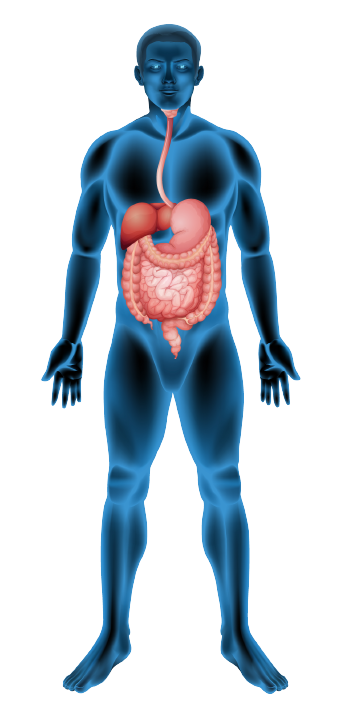
\includegraphics[width=.3\textwidth]{./imgs/cna1.jpg}
\end{wrapfigure}

No \textbf{sistema respiratório}, num circuito desde as fossas nasais até as
estruturas do pulmão, ocorre a inspiração de gás oxigênio e expiração de
gás carbônico. Enquanto o gás oxigênio é incorporado ao sangue, o gás
carbônico, produto de processos energéticos do organismo humano, é
eliminado. Nesse sistema, há o provimento de oxigênio que será utilizado
nos processos de divisão dos alimentos, gerando energia.

O transporte de oxigênio e de nutrientes é realizado pelo \textbf{sistema
circulatório}, que incorpora essas substâncias na corrente sanguínea,
transportada pelas veias e artérias e bombeadas para todas as partes do
corpo pelo coração. A atuação em conjunto com outros sistemas garante
que os tecidos do corpo humano sejam nutridos após a alimentação.}

\conteudo{
\includegraphics[width=.5\textwidth]{./imgs/cna2.jpg}
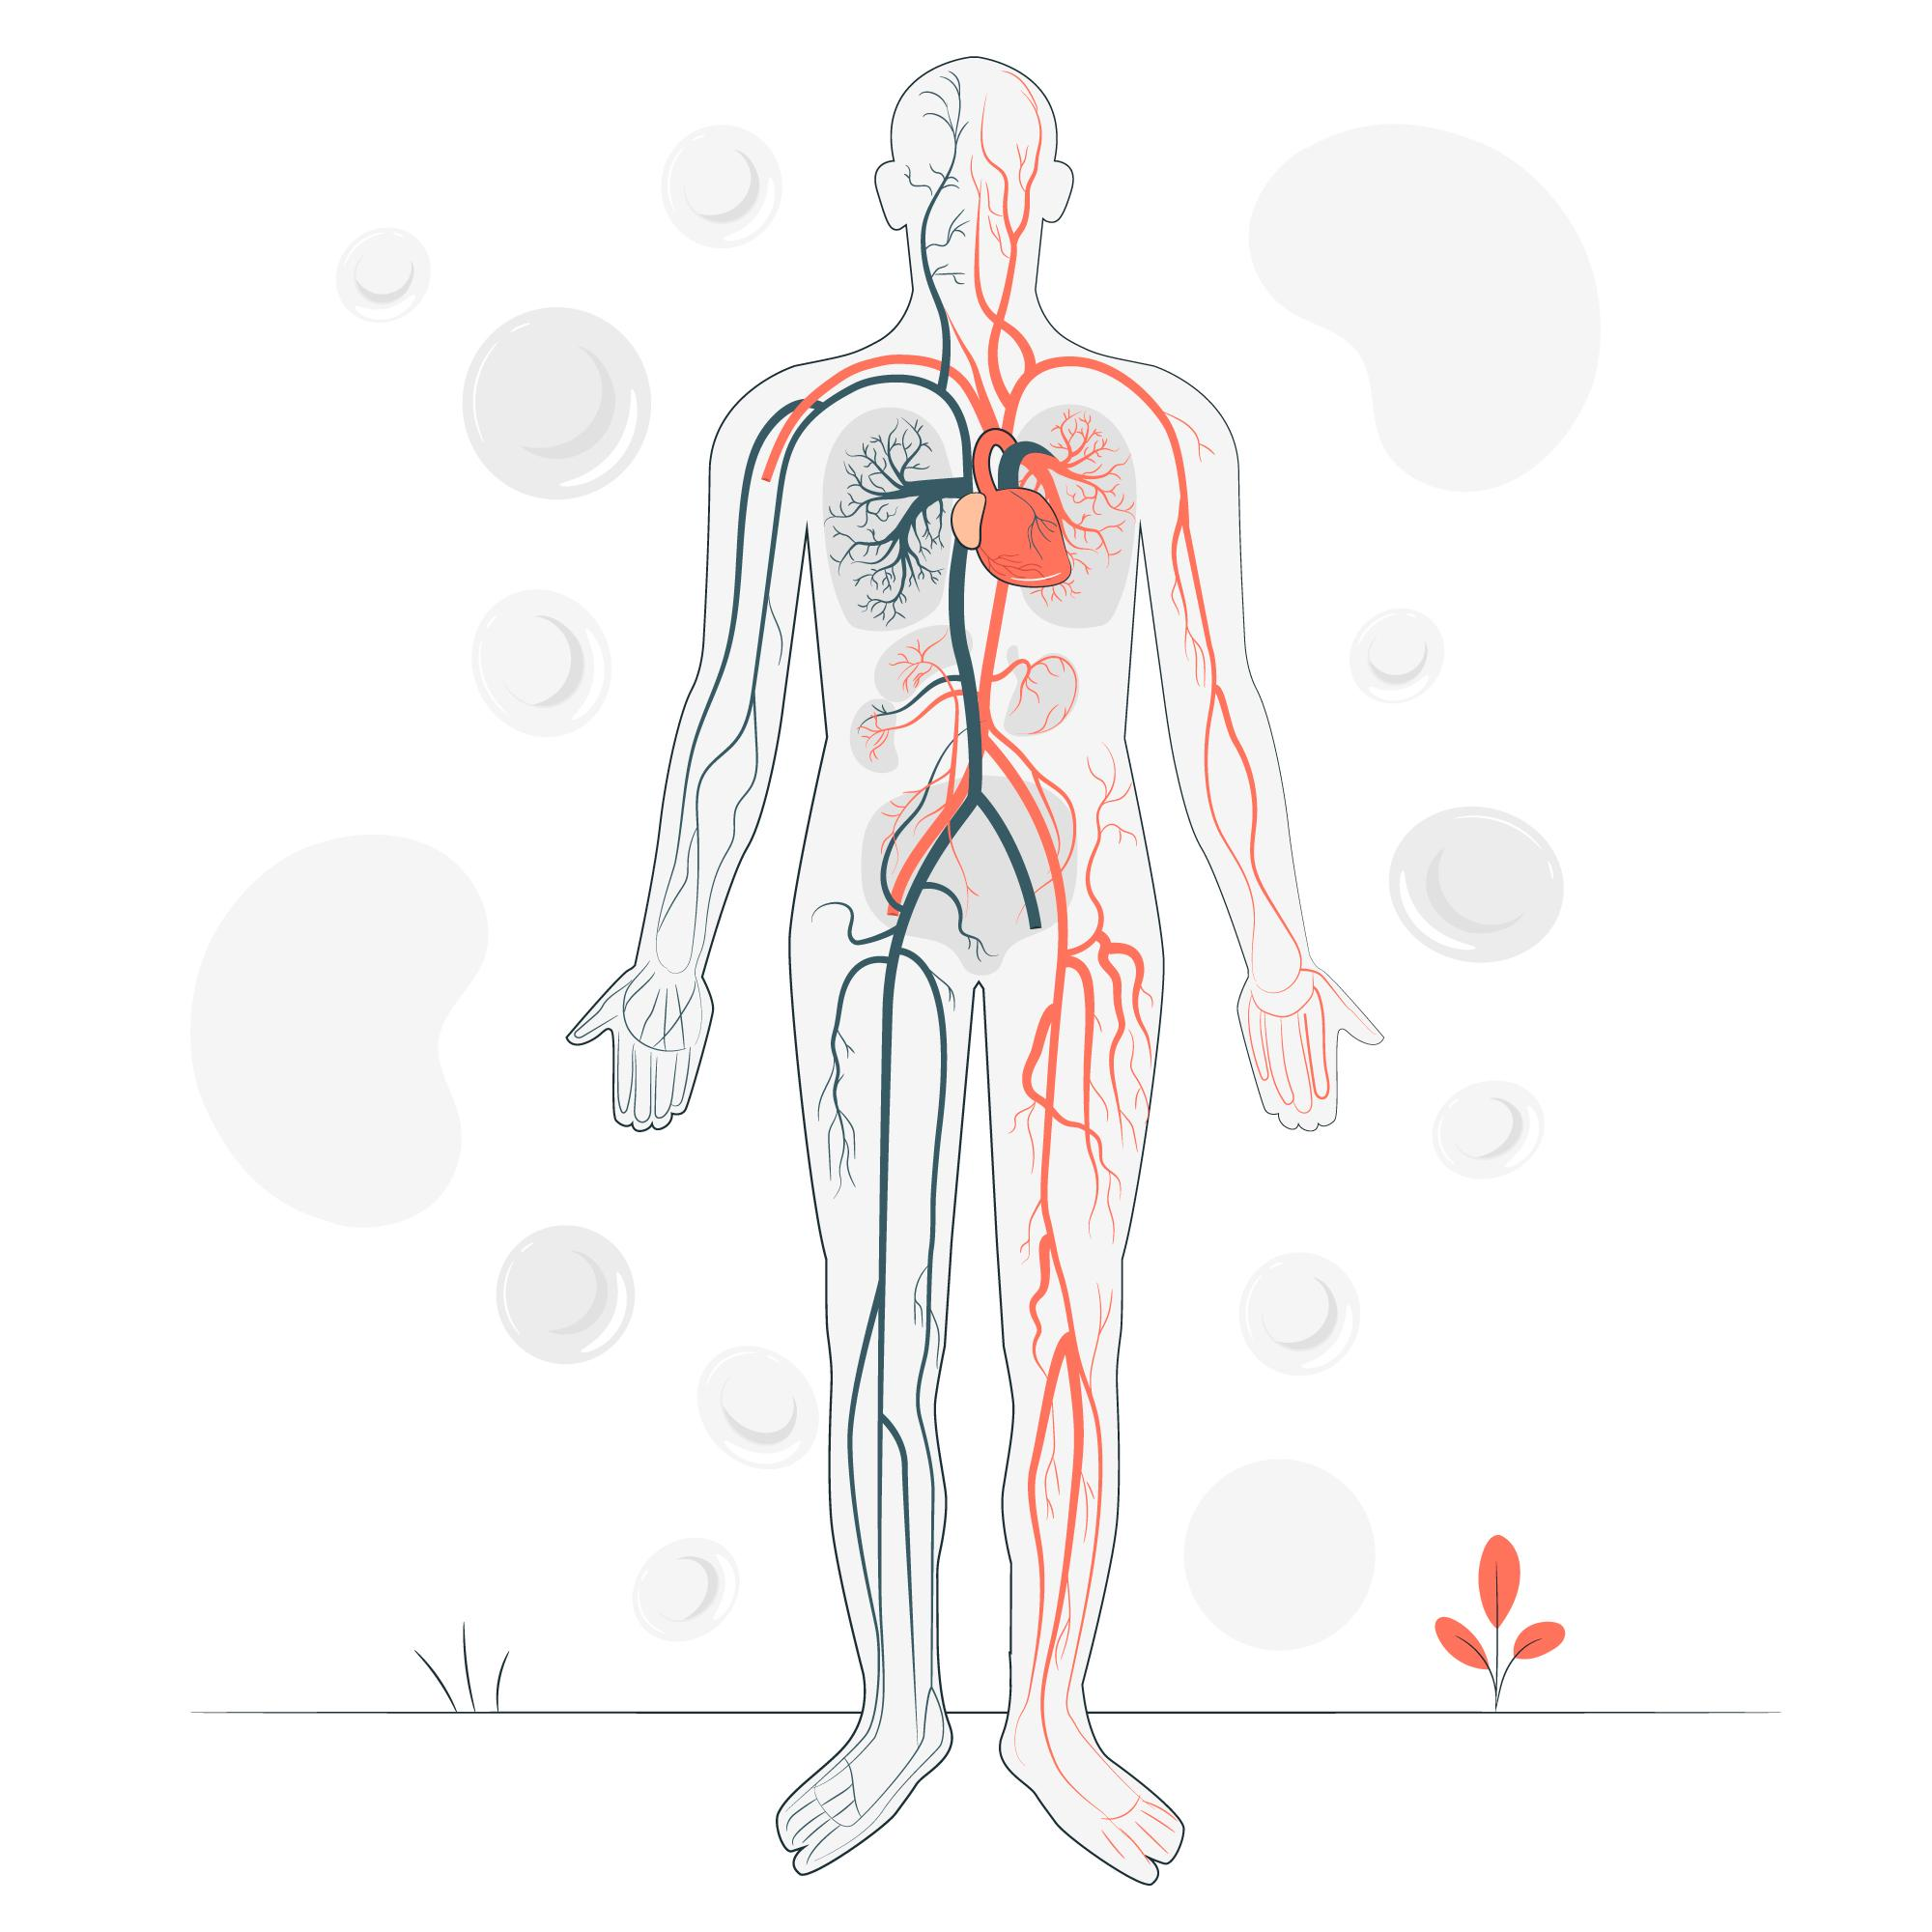
\includegraphics[width=.5\textwidth]{./imgs/cna3.jpg}

O funcionamento regular dos sistemas depende da alimentação saudável em
boas fontes de nutrientes. Alimentos com quantidades balanceadas de
carboidratos e gorduras, e ricos em fibras, proteínas e vitaminas são
essenciais para garantir que o máximo de nutrientes seja absorvido pelo
organismo, enquanto alimentos com calorias baseadas no excesso de
carboidratos e gorduras podem fazer com que o organismo se torne
deficiente em nutrientes e armazene gordura.

\begin{center}
\includegraphics[width=\textwidth]{./imgs/cna4.jpg}
\end{center}
}

\pagebreak
\section*{Atividades}

\num{1} Complete o texto com as palavras disponíveis.

\begin{mdframed}[linewidth=2pt,linecolor=salmao,backgroundcolor=salmao!20]
Boca \hfill Estômago \hfill Saliva \hfill Esôfago \hfill Quilo \hfill

\noindent{}Intestino delgado \hfill Quimo \hfill Intestino grosso \hfill Fezes \hfill Suco gástrico \hfill
\end{mdframed}

\begin{quote}
A digestão começa na \preencher{boca}, onde os alimentos ingeridos são triturados e envolvidos pela \preencher{saliva}, responsável por digerir o amido. O alimento é engolido e passa pelo \preencher{esôfago}, que faz movimentos peristálticos para empurrá-lo até o \preencher{estômago}. Depois, o alimento é amassado e se mistura com o \preencher{suco gástrico}.

Alguns nutrientes são absorvidos no estômago, enquanto o resto do bolo alimentar, chamado de \preencher{quimo} segue para o \preencher{intestino delgado}. Lá, parte dos nutrientes é aproveitada para a produção de energia, e o restante passa a ser chamado de \preencher{quilo}. No \preencher{intestino grosso}, a água e os nutrientes restantes são levados para o organismo, e a sobra é eliminada no formato de \preencher{fezes} pelo ânus.
\end{quote}

\num{2} O corpo humano precisa de energia para funcionar, e ela é
produzida com a junção de sistemas do organismo. Um desses sistemas, o
digestório, é responsável por processar os alimentos depois da ingestão.

\begin{escolha}
\item Como a alimentação participa da produção de energia para o corpo humano?\\
\reduline{A partir da alimentação, são absorvidos nutrientes
essenciais para a produção de energia pelo corpo humano, como proteínas,
fibras, vitaminas e gorduras.\hfill}
\linhas{2}

\item Como os bebês, apesar de não terem dentes, conseguem energia para
sobreviver?\\
\reduline{O aleitamento materno garante a nutrição dos bebês
por conter água e todos os nutrientes necessários para o desenvolvimento
saudável. Como eles não possuem dentes, teriam dificuldades em mastigar
alimentos maiores.\hfill}
\linhas{2}
\end{escolha}

\pagebreak
\num{3} Observe a imagem e responda.

\begin{figure}[htpb!]
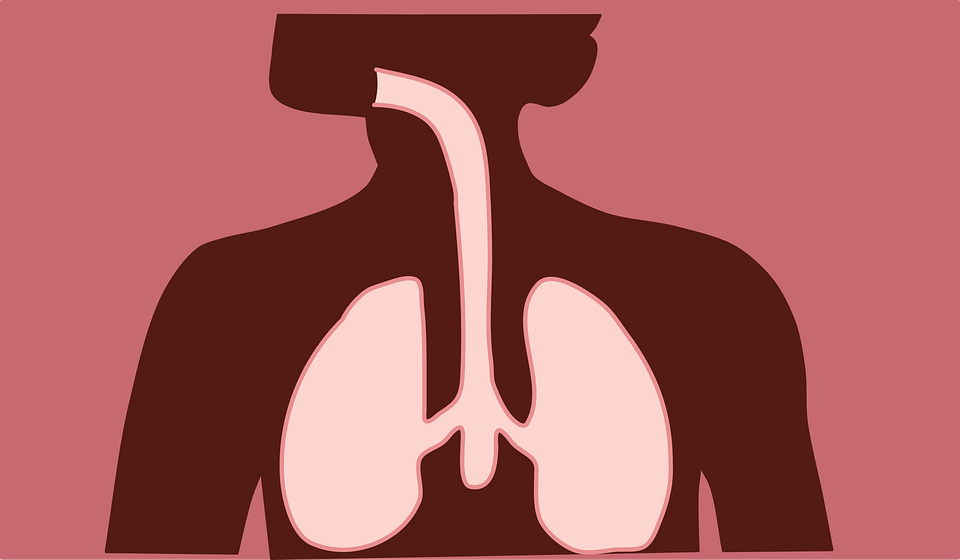
\includegraphics[width=\textwidth]{./imgs/img1.png}
\end{figure}
%\fonte{\emph{https://pixabay.com/pt/vectors/sistema-respirat\%c3\%b3rio-respirat\%c3\%b3rio-4869736/}}

\begin{escolha}
\item Quais são os órgãos representados na imagem?\\
\reduline{Os pulmões.\hfill}

\item Esses órgãos são os únicos responsáveis pela respiração humana?\\
\reduline{Os pulmões não são os únicos responsáveis pela respiração humana. Além deles, participam da respiração as
fossas nasais, faringe, traquéia, brônquios, bronquíolos, e alvéolos.\hfill}
\end{escolha}

\num{4} Durante a respiração, são realizados movimentos pelos
pulmões. Num deles, o nariz puxa o oxigênio do ar, os pulmões enchem e
ficam inflados, como um balão. Depois, esvaziam, com a liberação de gás
carbônico para o meio ambiente pelo nariz ou pela boca.

Como são chamados esses movimentos?

\reduline{Inspiração e Expiração.\hfill}
\linhas{2}

\pagebreak
\num{5} Complete a tabela com as informações corretas\medskip

\begin{tabular}{|l|l|l|}
\hline
\textbf{Processo} & \textbf{O que ocorre?} & \textbf{Onde ocorre?} \\ \hline
Troca gasosa & \begin{tabular}[c]{@{}l@{}}O oxigênio presente no ar\\ é inspirado e levado até\\ a corrente sanguínea,\\ enquanto o gás carbônico\\ é liberado via expiração\end{tabular} & \rosa{Pulmões} \\ \hline
Circulação sanguínea & \begin{tabular}[c]{@{}l@{}}\rosa{O sangue, concentrado em}\\ \rosa{oxigênio e nutrientes, é}\\ \rosa{bombeado para todas as}\\ \rosa{extremidades do corpo}\end{tabular} & \begin{tabular}[c]{@{}l@{}}Coração e\\ \rosa{vasos sanguíneos}\end{tabular} \\ \hline
\begin{tabular}[c]{@{}l@{}}Transporte de nutrientes,\\ como a glicose, para a célula\end{tabular} & \begin{tabular}[c]{@{}l@{}}\rosa{Os nutrientes são levados a}\\ \rosa{todos os órgãos, assim é gerada}\\ \rosa{energia ou se formam}\\ \rosa{reservas de gordura}\end{tabular} & No sistema circulatório \\ \hline
\end{tabular}\medskip

\num{6} Marque verdadeiro (V) ou falso (F):

\begin{boxlist}
\boxitem{V} Fazem parte do sistema circulatório o sangue, os vasos sanguíneos e o coração.

\boxitem{F} O sangue percorre todo o organismo, mas somente os pulmões transportam oxigênio.

\boxitem{V} O coração bombeia o sangue para todas as extremidades do corpo humano.

\boxitem{F} Os vasos sanguíneos podem se dilatar em temperaturas muito baixas.

\boxitem{V} Quando praticamos atividades físicas, o coração bombeia mais rápido 
o sangue contendo nutrientes e oxigênio por todo o organismo.
\end{boxlist}

% \coment{V, F, V, F, V. Na primeira afirmação falsa, afirma-se erroneamente
% que somente os pulmões transportam oxigênio, mas, na verdade, o sangue transporta
% oxigênio por todo o organismo. Na segunda afirmação falsa, afirma-se que os vasos 
% sanguíneos se dilatam em temperaturas baixas; na verdade, eles \textit{se contraem}
% em temperaturas muito baixas e \textit{se dilatam} com o aumento de temperatura.}

\num{7} Quando o corpo humano entra em contato com alguma doença e
desenvolve uma infecção, uma defesa é produzida e depois transportada
pelo sangue para combater o efeito das células malignas.

\begin{escolha}
\item Como são chamadas as células defensivas?\\
\reduline{As células de defesa capazes de combater uma infecção
são chamadas de anticorpos.\hfill}

\item Como essas células atuam?\\
\reduline{Os anticorpos são liberados na corrente sanguínea
pelo sistema imune após a detecção de um invasor pelos macrófagos e
atuam cercando as células malignas, destruindo-as.\hfill}

\item Qual a importância da vacinação para a produção de defesas do organismo?\\
\reduline{As vacinas estimulam a liberação de anticorpos para
combater uma infecção bem mais fraca, incapaz de deixar uma pessoa
doente. Mas, como o organismo possui memória imunológica, quando uma
infecção verdadeira ocorrer, os anticorpos estarão presentes e prontos
para combatê-la.\hfill}
\end{escolha}

\num{8} Marque a alternativa que descreve as funções do sistema circulatório corretamente.

\begin{escolha}
\item transporte de sangue por todas as extremidades do corpo, contendo
oxigênio, nutrientes e separação de toxinas para eliminação. \rosa{X}

\item filtragem de alimentos e do oxigênio respirado, e produção de gás
carbônico para expiração.

\item limpeza das impurezas do organismo, produção do suco gástrico e
remoção de células malignas do corpo.

\item regulagem das fezes produzidas pelo intestino grosso, separando
componentes a serem eliminados.
\end{escolha}

% A descrição das funções do sistema
% circulatório abarca o transporte de sangue por todo o corpo, contendo
% oxigênio e nutrientes, além da separação de toxinas a serem excretadas.
% Dessa maneira, o sistema circulatório se integra ao sistema respiratório
% e digestório. 
% Alternativa B: incorreta. O sistema circulatório não é responsável pela
% filtragem de alimentos. 
% Alternativa C: incorreta. O sistema circulatório não é responsável pela
% produção do suco gástrico
% Alternativa D: incorreta. O sistema circulatório não é responsável pela 
% regulagem das fezes.}

\num{9} A glicose é um dos principais nutrientes utilizados como
fonte de energia pelos seres humanos. Ela é aproveitada ao ser dividida
e convertida em outras substâncias para produção de energia. Entretanto,
algumas pessoas sofrem com o excesso da presença desse nutriente no
sangue.

Cite uma doença relacionada com o excesso de glicose na corrente
sanguínea.

\reduline{A doença relacionada com o excesso de glicose no
sangue é o \textit{diabetes mellitus}. Discuta com os alunos possíveis conhecimentos
que eles tenham sobre essa doença e explique que ela ocorre por conta da falha
no organismo em produzir a substância capaz de dividir ou quebrar a glicose.\hfill}
\linhas{4}

\pagebreak
\num{10} A figura a seguir representa um exemplo de pirâmide
alimentar.

\begin{figure}[htpb!]
\centering
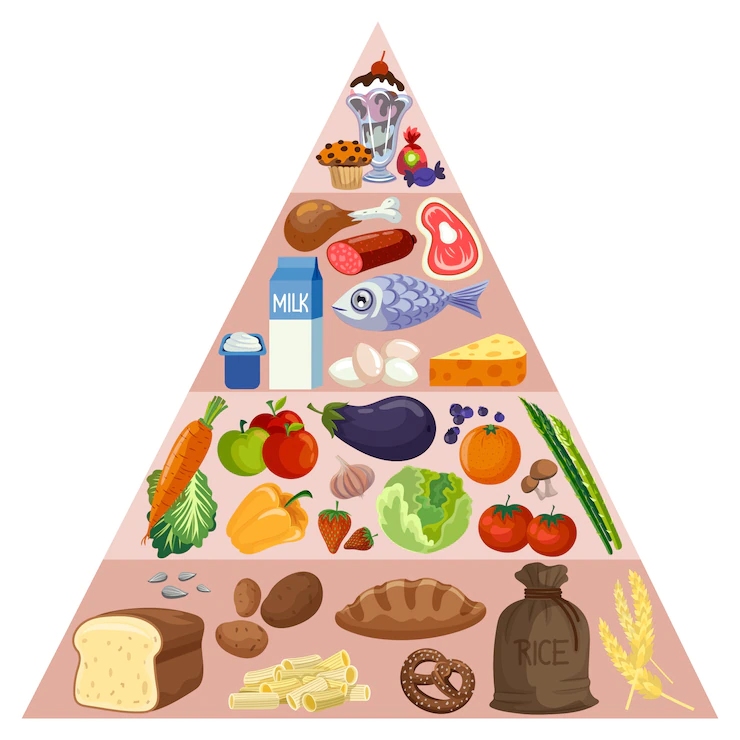
\includegraphics[width=.5\textwidth]{./imgs/img2.png}
\end{figure}

%\fonte{Imagem: Freepik / \emph{https://br.freepik.com/vetores-gratis/conceito-de-nutricao-de-design-de-piramide-alimentar\_7371729.htm\#query=pir\%C3\%A2mide\%20alimentar\&position=1\&from\_view=search\&track=ais}}

Observe a imagem e responda atentamente às perguntas:

\begin{escolha}
\item Por que alguns itens estão na base da pirâmide?\\
\reduline{Os alimentos da base da pirâmide representam as 
principais fontes de energia para o corpo humano, como os
carboidratos, em que são ricos os pães, bolos, batatas e grãos.\hfill}

\item Por que alguns itens estão no topo da pirâmide?\\
\reduline{Foram colocados no topo da pirâmide os alimentos de menor
importância para uma alimentação saudável e, sugestivamente, de menor
valor nutricional. São eles os doces, chocolates, frituras e demais
alimentos processados.\hfill}

\item Qual a recomendação para uma alimentação saudável, observando 
os alimentos da pirâmide?\\
\reduline{Observa-se que a alimentação deve ser balanceada, sem
exagerar em nenhum dos níveis da pirâmide, mas composta principalmente
pelos alimentos da base, com participação fundamental, também, de outras
classes representadas, como legumes, laticínios, peixes e carnes, que são fontes
de proteína.\hfill}
\end{escolha}

\num{11} Durante um processo de reeducação alimentar, uma pessoa
estimou que precisava consumir cerca de 1800 kcal por dia, resultado
compatível com a sua altura e peso. Para controlar a alimentação, anotou
as informações de alguns alimentos.

\begin{center}
\noindent\resizebox{\textwidth}{!}{
\begin{tabular}{@{}llllll@{}}
        \toprule
        \textbf{Alimento (porção de 100g)} & \textbf{Energia (calorias)} & \textbf{Carboidratos} & \textbf{Gorduras} & \textbf{Proteínas} & \textbf{Fibra alimentar} \\ \midrule
        Batata frita & 250kcal & 33g & 12g & 4g & 3g \\
        Batata cozida & 50kcal & 12g & 0g & 1g & 1g \\
        Biscoito doce & 440kcal & 76g & 11g & 8g & 3g \\
        Banana prata & 105kcal & 26g & 0g & 1g & 2g \\
        Salada de legumes & 35kcal & 7g & 0g & 2g & 3g \\
        Pizza calabresa & 260kcal & 33g & 10g & 10g & 2g \\
        Hambúrguer fast food & 261kcal & 30g & 10g & 13g & 1g \\
        Risoto de legumes com arroz & 140kcal & 14g & 8g & 3g & 2g \\ \bottomrule
    \end{tabular}
}
\end{center}

\fonte{Tabela Brasileira de Composição de Alimentos (TBCA) da Universidade de São Paulo (USP). Disponível em: \emph{http://www.fcf.usp.br/tbca}. Acesso em: 29 mar.23}

A pessoa notou que, mesmo se a alimentação diária fosse baseada em
alimentos como batata frita, biscoito doce, pizza e hambúrguer \textit{fast
food}, não ultrapassaria as necessidades calóricas diárias.

\begin{escolha}
\item Apenas o controle da quantidade de calorias ingeridas é
suficiente para manter uma alimentação saudável?\\
\reduline{O controle da quantidade de calorias ingeridas \textbf{não é}
suficiente para manter uma alimentação saudável. Além das calorias ingeridas,
a proporção de nutrientes é fundamental para o equilíbrio da alimentação. 
Batata frita, biscoito doce, pizza e hambúrguer \textit{fast food} são 
alimentos com grande quantidade de carboidratos e gorduras, e recomenda-se
que não haja exagero na ingestão desses nutrientes para a manutenção da saúde.\hfill}

\item Como uma dieta balanceada deve funcionar?\\
\reduline{Uma dieta balanceada deve equilibrar o consumo de
carboidratos, gorduras, proteínas e fibras, de acordo com as
necessidades de cada indivíduo. A alimentação com as chamadas calorias
podres, como alimentos ultraprocessados, deve ser reduzida.\hfill}

\pagebreak
\item Monte, no espaço abaixo, um cardápio para uma alimentação
com base nos alimentos da tabela. Pesquise outros alimentos importantes
para o consumo diário, sem esquecer de anotar as informações
nutricionais.

\begin{mdframed}[linewidth=2pt,linecolor=salmao,roundcorner=20pt]
\coment{Espera-se que os alunos observem as informações
disponíveis em rótulos nutricionais para construir um cardápio
equilibrado, sem exageros ou cortes radicais.}
\vspace{7cm}
\end{mdframed}
\end{escolha}

\section*{Treino}

\num{1}

\begin{myquote}
A alimentação é uma fonte essencial de nutrientes para o
corpo humano. Diversos órgãos necessitam da energia gerada a partir da
digestão, na qual ocorre a separação do que pode ser aproveitado pelo organismo
e do que deve ser descartado. Os nutrientes, como a glicose e as
proteínas, são levados para todas as extremidades do corpo e,
incorporados aos músculos, estocados na forma de gordura ou degradados.
\end{myquote}

O transporte dessas substâncias é realizado no

\begin{escolha}
\item sistema circulatório.

\item sistema digestório.

\item sistema respiratório.

\item sistema reprodutivo.
\end{escolha}


\pagebreak
\num{2}

\begin{myquote}
Segundo dados da Fiocruz e da UNICEF, em 2022 a taxa de
vacinação infantil no Brasil sofreu uma queda brusca: a média de 90 a 95\%,
registrada nas últimas décadas, caiu para cerca de 71,49\%. Esse processo
foi acelerado nos últimos anos, aumentando o risco do retorno de doenças
que já tinham sido erradicadas, ou seja, que tinham desaparecido por conta
da vacinação. 
\end{myquote}

A falta de vacinação de doenças erradicadas põe uma pessoa em risco pois

\begin{escolha}
\item a estrutura de defesa do corpo só existe com a vacina.

\item a vacina regula sistemas do corpo humano.

\item o organismo fica mais vulnerável a infecções.

\item o sangue precisa levar a vacina para os locais infectados.
\end{escolha}



\num{3} Leia o texto.

\begin{myquote}
No final das contas, as calorias importam, sim, mas nunca sozinhas.
Nosso corpo precisa ser nutrido, algo que algodão doce, batata frita e
outros alimentos ultraprocessados não farão por nós. Eles não estão
proibidos, mas devem ser consumidos com moderação.

\fonte{Marcella Garcez. Veja Saúde. O que a contagem de calorias pode esconder.
Disponível em:
\emph{https://saude.abril.com.br/coluna/com-a-palavra/o-que-a-contagem-de-calorias-pode-esconder/}.
Acesso em: 29 mar. 2023.}
\end{myquote}

Uma alimentação balanceada deve considerar fatores além da contagem de
calorias, pois

\begin{escolha}
\item as informações dos rótulos nutricionais não são estimativas confiáveis.

\item as necessidades calóricas variam de corpo a corpo.

\item os demais nutrientes, como carboidratos, gorduras e proteínas, devem ser observados.

\item os alimentos ultraprocessados também podem ser benéficos ao organismo.
\end{escolha}



\chapter{Sistema solar}
\markboth{Módulo 3}{}

\vspace*{-1cm}
\enlargethispage{2\baselineskip}

\section*{Eixo de conhecimento do SAEB}

\begin{itemize}
	\item Terra e universo.
\end{itemize}

\subsection{Habilidades da BNCC}

\begin{itemize}
\item EF05CI11, EF05CI12.
\end{itemize}

%Felipe Augusto: aqui fiz a seguinte padronização:
% Terra, Lua e Sol em letras maiúsculas, salvo em referências genéricas
% As fases da lua estão em letras minúsculas
% Os movimentos de Rotação, Translação e Revolução estão em maiúsculas
% Hemisfério Sul e Hemisfério Norte estão em maiúsculas

\conteudo{
\begin{wrapfigure}{l}{.4\textwidth}
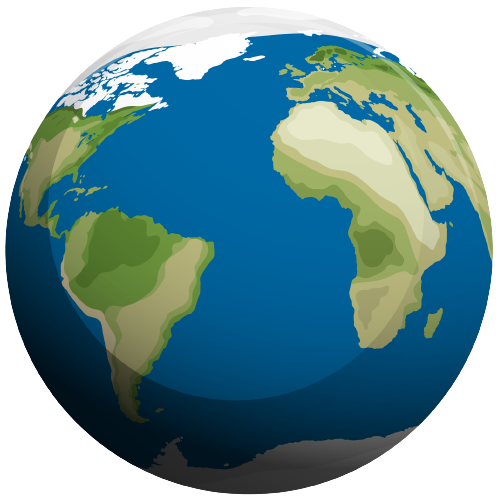
\includegraphics[width=.4\textwidth]{./imgs/img18.jpg}
\end{wrapfigure}
%caption{https://br.freepik.com/vetores-gratis/terra-isolada-em-branco_13774164.htm#query=Planeta%20Terra&position=4&from_view=search&track=ais}
A Terra é um corpo celeste que faz parte do sistema solar.
Os movimentos de nosso planeta em torno do Sol e do próprio eixo 
garantem a manutenção da sobrevivência dos seres humanos. Essa complexa 
dinâmica regula a duração dos dias e das noites, além dos fusos horários
em diferentes localidades e estações do ano, nos Hemisférios Sul e Norte.

\begin{wrapfigure}{l}{.5\textwidth}
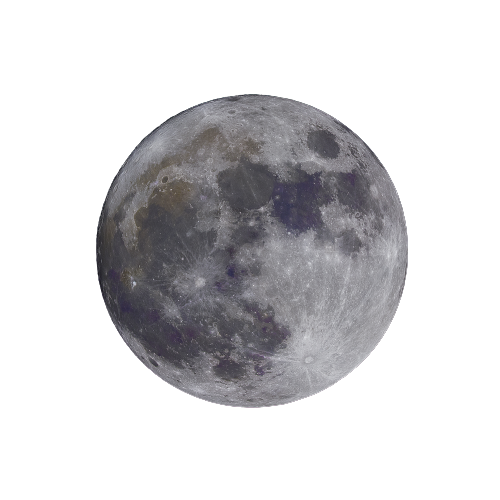
\includegraphics[width=.5\textwidth]{./imgs/img19.jpg}
\end{wrapfigure}
%caption{https://br.freepik.com/fotos-gratis/closeup-tiro-da-lua-isolado-em-um-fundo-preto-otimo-para-artigos-sobre-espaco_9283057.htm#query=terra%20lua&position=14&from_view=search&track=ais}

A Lua é um satélite natural que também realiza movimentos constantes 
em torno do Sol, da Terra e do seu próprio eixo. Enquanto o Sol é visível
durante o dia, a Lua pode ser observada à noite, a depender da posição
que ocupa em relação aos outros dois corpos celestes.

Como a movimentação da Lua em torno da Terra é periódica, suas formas
aparentes representam quatro fases de um ciclo lunar: lua crescente,
lua cheia, lua minguante e lua nova. Essas diferentes fases contribuem 
para a compreensão de fenômenos naturais, como marés e eclipses, além de
se relacionarem a costumes e culturas milenares, que duram até hoje.}

\section*{Atividades}

\num{1} O planeta Terra é um corpo celeste que se movimenta em
torno de seu próprio eixo. O movimento é importante para todos os seres
vivos, pois garante a existência dos dias e das noites.

\begin{escolha}
\item Qual o nome desse movimento?\\
\reduline{Rotação.\hfill}

\item Qual a duração desse movimento?\\
\reduline{23 horas e 56 minutos.\hfill}
\end{escolha}

\num{2} Dois amigos decidiram observar o céu em diferentes horas do
dia, e anotaram suas impressões sobre os fenômenos ocorridos.

\begin{mdframed}[linewidth=5pt,linecolor=salmao!20,backgroundcolor=salmao!20,roundcorner=20pt]
\textbf{Observação 1}\\
Está muito calor, mas consigo ver as nuvens
do céu. Elas estão se movimentando a todo momento, e o restante
da Terra fica parado.
\end{mdframed}

\begin{mdframed}[linewidth=5pt,linecolor=azul!20,backgroundcolor=azul!20,roundcorner=20pt]
\textbf{Observação 2}\\
O movimento das estrelas, caso eu esteja
parado observando, é aparente. Mas, na verdade, a Terra está se
movimentando junto comigo, e não só as estrelas!
\end{mdframed}

\noindent{}Os dois trocaram suas observações e perceberam que tinham noções
diferentes sobre o que foi visto.

\begin{escolha}
\item Qual das duas observações está correta?\\
\reduline{A observação correta é a de número 2, pois nela está descrito 
corretamente o movimento de rotação da Terra. Para um observador que
se mantém parado, observando as estrelas de um ponto fixo, a sensação
de que só as estrelas estão se movimentando é ilusória. Na verdade, o
movimento é do planeta, inclusive do observador.\hfill}

\item Qual o erro da observação incorreta?\\
\reduline{O erro da observação 1 é imaginar que a Terra não está se
movimentando devido ao movimento aparente das nuvens. Por mais que
não seja perceptível para o observador, o movimento de Rotação está 
acontecendo.\hfill}
\end{escolha}

\num{3} Observe a imagem.

%(pedido do autor) IMAGEM DO SOL CONTRA UM FUNDO ESCURO, COM QUATRO VERSÕES DA TERRA REALIZANDO O MOVIMENTO DE VOLTA EM TORNO DO SOL. INDICAR O SENTIDO DA VOLTA COM SETAS, BEM COMO TOMAR CUIDADO PARA MOSTRAR A TERRA EM POSIÇÕES DIFERENTES; SE POSSÍVEL, DEMONSTRAR QUE A TERRA ESTÁ GIRANDO EM TORNO DE SEU PRÓPRIO EIXO. PEGUEI UMA IMAGEM DA INTERNET COMO REFERÊNCIA, MAS NÃO ACHEI NENHUMA LIVRE DE DIREITOS.

\begin{figure}[htpb!]
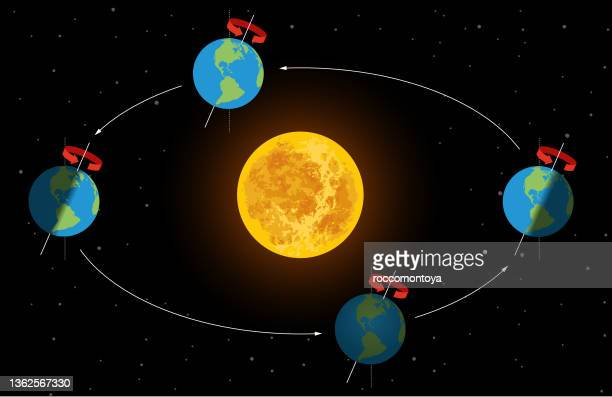
\includegraphics[width=\textwidth]{./imgs/img3.png}
\end{figure}
%Fonte: Getty Images / \href{https://www.gettyimages.com.br/fotos/earth-sun-rotation}{\emph{https://www.gettyimages.com.br/fotos/earth-sun-rotation}}

\begin{escolha}
\item Qual o nome do movimento ilustrado?\\
\reduline{Translação.\hfill}

\item O movimento da Rotação ocorre ao mesmo tempo que o movimento indicado na imagem?\\
\reduline{Os movimentos de Rotação e Translação são simultâneos:
enquanto cada Rotação completa descreve um dia de aproximadamente
24 horas, as 365 rotações ocorrem durante a volta da Terra ao redor
do sol.\hfill}
\end{escolha}

\num{4} Os anos terrestres duram aproximadamente 365 dias, 5 horas
e 48 minutos. O período de um ano nesse ciclo representa a movimentação
da Terra em torno do Sol, sendo assim, a volta só termina no último dia.

Por que, a cada quatro anos, ocorre um ano bissexto?

\reduline{As horas e os minutos acumulados durante as voltas da
Terra em um ano regular totalizam, em quatro anos, a duração aproximada
de um novo dia de 24 horas. Portanto, nesse período ocorre um ano
bissexto, com um dia a mais no mês de Fevereiro.\hfill}

\num{5} São conhecidas 4 estações do ano: verão, outono, inverno e
primavera. No verão, os dias são mais iluminados e mais quentes; no
outono, caem as folhas e temperaturas; no inverno, predomina o frio; na
primavera, crescem as folhas.

\begin{escolha}
\item Qual a relação entre movimento da Terra e as estações do ano?\\
\reduline{A variação das estações do ano ocorre de acordo com a
posição da Terra em relação ao sol e aos hemisférios e com a inclinação
do eixo de rotação. Durante o movimento de Translação, ocorrem as estações
conhecidas, pois cada uma delas descreve um quarto da movimentação do
planeta em torno do sol.\hfill}

\item Como os movimentos da Terra determinam o clima em todas as regiões do planeta?\\
\reduline{De acordo com a distribuição da energia solar, em
forma de luz e calor, os movimentos de Rotação e Translação determinam
um padrão climático para as regiões da Terra nas respectivas estações do
ano. Fatores regionais variados podem modificar o clima esperado e
característico da cada região.\hfill}
\end{escolha}

\num{6} Quando é dia em São Paulo, no Brasil, é noite em Osaka, no
Japão. Esse fenômeno pode ser representado por duas imagens comparando
os centros comerciais dessas cidades:

\pagebreak
\begin{figure}[htpb!]
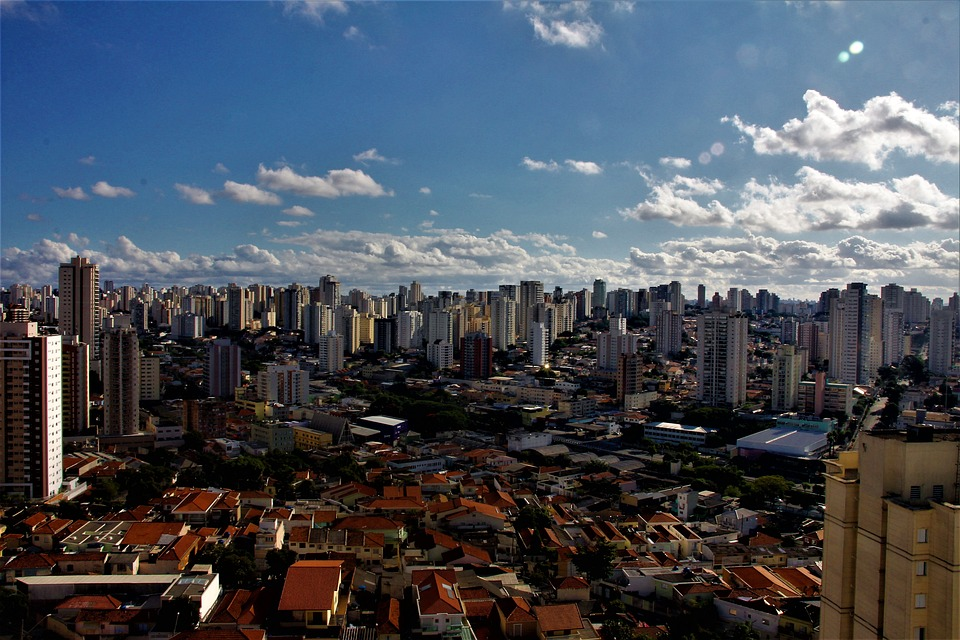
\includegraphics[width=.5\textwidth]{./imgs/img4.png}

\includegraphics[width=.5\textwidth]{./imgs/img5.png}
\end{figure}
%Imagens do Pixabay
%Imagem 1: \href{https://pixabay.com/pt/photos/s\%c3\%a3o-paulo-dia-da-sa\%c3\%bade-brasil-4958304/}{\emph{https://pixabay.com/pt/photos/s\%c3\%a3o-paulo-dia-da-sa\%c3\%bade-brasil-4958304/}}
%Imagem 2: \href{https://pixabay.com/pt/photos/jap\%c3\%a3o-osaka-pedestres-cruzando-2014616/}{\emph{https://pixabay.com/pt/photos/jap\%c3\%a3o-osaka-pedestres-cruzando-2014616/}}

\noindent{}Como é possível, ao mesmo tempo, que numa parte do planeta seja dia,
enquanto em outra seja noite?

\reduline{A Terra, durante o movimento de Rotação, não recebe a
luz solar da mesma maneira em todos os pontos de sua superfície
esférica. Enquanto em algumas regiões é dia, em outras, em lugares
opostos, não há incidência da luz solar. O Brasil e o Japão tem fusos
horários muito distintos por conta desse fenômeno.\hfill}

\num{7} Complete as duas lacunas a seguir.

\begin{quote}
No solstício de verão, a luz solar incide com \preencher{maior\hspace{.5cm}} intensidade em um dos hemisférios da terra. A principal característica desse período é a \preencher{maior\hspace{.5cm}} duração dos dias.
\end{quote}

\num{8} Relacione os itens:

{\setlength{\columnsep}{-5cm}
\begin{multicols}{1}
1. Solstício de inverno.

2. Equinócio.

3. Rotação da Lua.

4. Solstício de verão.

5. Revolução da Lua.

6. Rotação da Terra.

7. Translação da Lua.

\columnbreak

({\rosa{4}}) os dias duram mais do que as noites.

({\rosa{3}}) movimento da Lua em torno do seu próprio eixo.

({\rosa{1}}) as noites duram mais do que os dias.

({\rosa{7}}) movimento da Lua em torno do Sol.

({\rosa{2}}) os dias e as noites possuem a mesma duração.

({\rosa{6}}) movimento da Terra em torno do seu próprio eixo.

({\rosa{5}}) giro da Lua em torno da Terra.
\end{multicols}
}

\num{9} Marque verdadeiro (V) ou falso (F)

\begin{boxlist}
\boxitem{V} A Lua é um satélite natural da Terra.

\boxitem{F} A luz emitida pela Lua é responsável por iluminar as noites.

\boxitem{V} Rotação, Revolução e Translação são movimentos realizados pela Lua.

\boxitem{V} Sem a Lua, as noites seriam totalmente escuras.
\end{boxlist}

% \coment{V, F, V, V. A segunda afirmação é falsa, porque a luz da Lua é
% reflexo da luz solar; a rigor, portanto, a iluminação noturna não é
% \textit{emitida} pela Lua, mas pelo Sol.}

\num{10} Apesar de não emitir luz própria, a Lua é capaz de
refletir a luz solar. Por conta desse fenômeno, conseguimos entender as
fases lunares de acordo com o que é visível na Terra. Quando a Terra está
entre a Lua e o Sol, temos a lua cheia, na qual o satélite natural é
totalmente visível a partir da superfície terrestre. Nessa mesma fase,
ocorrem os chamados eclipses lunares.

O que são eclipses lunares?

\reduline{São fenômenos astronômicos que ocorrem quando a
sombra do planeta Terra, posicionado entre a Lua e o Sol, bloqueia a
chegada de luz na superfície lunar, ou seja, quando há um alinhamento
perfeito entre Terra, Sol e Lua.\hfill}

\num{11} Um cientista observou as noites durante uma semana, a fim
de entender as fases da Lua, e registrou as seguintes ocorrências:

\begin{longtable}[]{@{}ll@{}}
\toprule
\textbf{Dias} & \textbf{Descrição}\tabularnewline
1 e 2 & Tamanho da lua pequeno, imagem côncava e
decrescente.\tabularnewline
2 e 3 & Lua não visível.\tabularnewline
3 e 4 & Lua não visível.\tabularnewline
4 e 5 & Pequena parte da lua visível.\tabularnewline
5 e 6 & Pequena parte da lua visível.\tabularnewline
6 e 7 & Pequena parte da lua visível. Imagem côncava e
crescente.\tabularnewline
\bottomrule
\end{longtable}

Mesmo que não observasse todos os dias, a que conclusão o cientista
poderia chegar sobre as fases da Lua nos três primeiros dias?

\reduline{O cientista teria percebido que a fase da Lua nos
dois primeiros dias era a lua minguante, enquanto no dia seguinte,
quando não havia lua visível, a indicação era a de lua nova. Nessa
situação, a Lua se põe entre a Terra e o Sol, e, caso fosse um período
sinódico, se manteria nessa posição por até 8 dias.\hfill}

\conteudo{Os ciclos lunares sinódicos
duram cerca de 29,5 dias, descrevendo um mês lunar. É nesse período de
tempo que se considera um ciclo lunar completo, no qual as fases da Lua
duram em torno de 7 a 8 dias.

Já os ciclos lunares siderais duram aproximadamente 27,3 dias. Algumas
fases da Lua podem ser incompletas, por conta dos movimentos de Rotação
e Revolução realizados pela Lua.}

\pagebreak
\num{12} Observe a imagem que descreve o ciclo lunar em Janeiro de 2023:

%\textbf{Calendário: 1-31/01/2023}
\begin{figure}[htpb!]
\centering
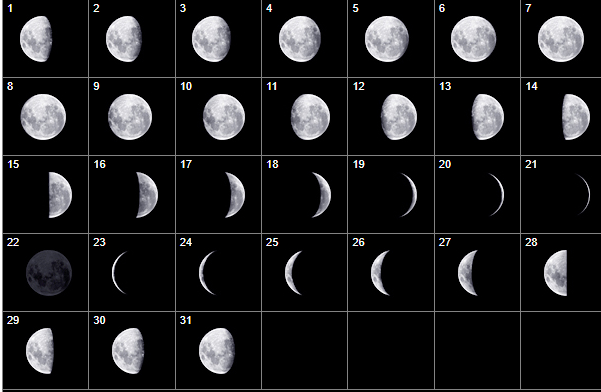
\includegraphics[width=\textwidth]{./imgs/img6.png}
\end{figure}
%\textbf{Fonte:} Moon Connection \textbf{/ \href{https://www.moonconnection.com/moon_phases_calendar.phtml}{\emph{https://www.moonconnection.com/moon\_phases\_calendar.phtml}}}

\begin{escolha}
\item Complete a tabela abaixo para cada uma das quatro fases da Lua:

\begin{center}
\begin{tabular}{|l|l|}
\hline
\textbf{Fase} & \textbf{Dia} \\ \hline
\rosa{Lua cheia} & 7 \\ \hline
Lua minguante & \begin{tabular}[c]{@{}l@{}}\rosa{Mais perceptível nos dias}\\ \rosa{13, 14, 15, 16, 17, 18, 19, 20, 21}\\ \rosa{(Qualquer um desses pode ser citado)}\end{tabular} \\ \hline
\rosa{Lua nova} & 22 \\ \hline
\rosa{Lua crescente} & 27 \\ \hline
\end{tabular}
\end{center}

\item Qual dos ciclos da Lua pôde ser observado em janeiro de 2023?\\
\reduline{Em janeiro de 2023 ocorreu o ciclo lunar sideral, pois se
observaram fases da Lua
incompletas, como no caso da lua nova. Esse ciclo dura, aproximadamente,
27,3 dias, tendo se iniciado entre 5 e 7 de janeiro de 2023 e encerrado,
provavelmente, entre 31 de janeiro de 2023 e 02 de fevereiro de 2023.\hfill}
\end{escolha}

\pagebreak
\section*{Treino}

\num{1} No mês de fevereiro, às 16h de uma tarde ensolarada no
Brasil, o Japão está mergulhado na escuridão da madrugada. Ao mesmo
tempo, um novo dia começa na Austrália, enquanto, nos
Estados Unidos, faz frio.

Esse fenômeno é explicado pela

\begin{escolha}
\item irradiação do sol nas regiões da Terra.

\item diminuição das camadas de proteção solar.

\item elevação do nível d'água no Hemisfério Sul.

\item consolidação das mudanças climáticas na superfície terrestre.
\end{escolha}


\num{2} Terra e Lua estão sempre em movimento. O planeta gira em
torno do próprio eixo e completa uma Rotação em torno do sol em 365
dias. A Lua, além de girar em torno do próprio eixo, gira em torno da
Terra e também em torno do Sol durante o ano.

Quais são os movimentos descritos no texto?

\begin{escolha}
\item Rotação terrestre, Revolução terrestre, Rotação lunar e Translação lunar.

\item Revolução terrestre, Rotação lunar, Translação lunar e Revolução lunar

\item Rotação terrestre, Translação terrestre, Rotação lunar, Translação lunar e Revolução lunar.

\item Rotação solar, Translação terrestre, Rotação lunar e Revolução lunar.
\end{escolha}

\num{3} É também no verão que, ao mesmo tempo em que o Sol nasce mais cedo, ele
também se põe mais tarde, o que faz com que os dias sejam mais longos. A
latitude — a distância do local em que se está até a Linha do Equador
— determina se um dia é mais curto ou mais longo. Quando mais próxima
uma localidade estiver desse marco, menos variações vai sofrer com as
estações do ano.

\fonte{Ivana Fontes. Portal Terra. Por que o dia escurece mais tarde no verão?.
Disponível em:
\emph{https://shorturl.at/jvFRX}.
Acesso em: 29 mar. 2023.}

O fenômeno que inicia a estação do ano citada no texto é chamado de

\begin{multicols}{2}
\begin{escolha}
\item equinócio de primavera.

\item solstício de verão.

\item solstício de inverno.

\item equinócio de outono.
\end{escolha}
\end{multicols}




%REFERÊNCIAS

%DÂNGELO, J. G.; FATTINI, C. A. Anatomia humana sistêmica e segmentar. 2a
%ed. Rio de Janeiro: Atheneu, 2011.
%
%FERREIRA, P. F.; LEITE, C. A FORMA E OS MOVIMENTOS DA TERRA: PERCEPÇÕES
%DE PROFESSORES ACERCA DAS RELAÇÕES ENTRE OBSERVAÇÃO COTIDIANA E OS
%MODELOS CIENTÍFICOS. \textbf{Revista Latino-Americana de Educação em
%Astronomia - RELEA}, n. 19, p. 123-146, 2015
%
%GONÇALVES, P. C. DA S.; BRETONES, P. S.. O ensino sobre a Lua e suas
%fases: uma proposta observacional para os Anos Iniciais do Ensino
%Fundamental. \textbf{Ensaio Pesquisa em Educação em Ciências (Belo
%Horizonte)}, v. 23, n. Ens. Pesqui. Educ. Ciênc. (Belo Horizonte), 2021.
%
%HORNIK, G. G.; HENRIQUE, A.; HORNIK, E. N. H\textsubscript{2}O - O Ciclo
%da Vida. Alfenas: Independente, 2016.
%
%MIRANDA, R. A. C.; OLIVEIRA, M. V. S.; SILVA, D. F. CICLO HIDROLÓGICO
%PLANETÁRIO: abordagens e Conceitos. \textbf{Geo UERJ}, Rio de Janeiro -
%RJ, ano 12, v. 1, n. 21, 2010.
%
%TONEL, A. P.; MARRANGHELLO, G. F.. O movimento aparente da Lua. Revista
%Brasileira de Ensino de Física, v. 35, n. \textbf{Rev. Bras. Ensino
%Fís.}, 2013 35(2), abr. 2013.

\pagebreak